\documentclass{article}
\usepackage{amsmath}
\usepackage{mathtools}
\usepackage{gensymb}
\usepackage[a4paper,inner=1.5cm,outer=1.5cm,top=2cm,bottom=0.5cm]{geometry} 
\usepackage{xcolor}
\usepackage{tikz}
\usepackage{multicol}
\usepackage{pgfplots}
\usetikzlibrary{intersections}
\usetikzlibrary{intersections,calc,angles,quotes}
\usetikzlibrary{calc,angles,positioning,intersections,quotes,decorations.markings}
\usepackage{tkz-euclide}
\usetikzlibrary{backgrounds}
\usetikzlibrary{calc,through}
\usetikzlibrary{angles}
\usetikzlibrary{fadings}
\usetikzlibrary{shapes.geometric}
\usetikzlibrary{shapes.symbols}
\usepackage{draftwatermark}
\usepackage{mathptmx}

\SetWatermarkText{\textcolor{black!30}{Mathema Shukur}}
\SetWatermarkFontSize{2 cm}
\usepackage[utf8]{inputenc}
\usepackage{fontspec}

\setmainfont{[Kalpurush.ttf]}
\newfontface{\en}{[Arial.ttf]} %%this is optional, if you want to use a secondary font. Any english font is supported
\newlength\Radius
\setlength\Radius{4cm}
\begin{document} 
	\Large
	\textcolor{red}{Welcome To} 
	\\
	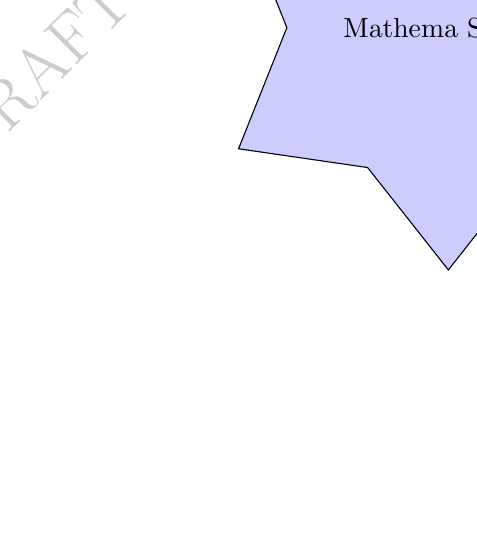
\begin{tikzpicture}
		\tikz \node [fill=blue!20,star,star points=6,draw] {Mathema Shukur };
	\end{tikzpicture}
	\\
	যাদের জন্যে প্রযোজ্যঃ  	\textcolor{magenta}{একাদশ ও দ্বাদশ শ্রেণীর শিক্ষার্থী} \\
	বিষয়ঃ \textcolor{magenta}{উচ্চতর গণিত ১ম পত্র} \\
	অধ্যায়ঃ \textcolor{magenta}{৩-সরলরেখা}\\ 
	Subtopicঃ  \textcolor{magenta}{ কার্তেসীয় (x,y)  স্থানাঙ্ক নির্ণয় করা }\\
	\\
	\\
	$\textcolor{blue}{x=r\,\,\cos \theta}$ , $\textcolor{blue}{y=r\,\,\sin \theta}$ \\
	\\
	(১) যশোর বোর্ড-২০১৯\\
	কোনো বিন্দুর পোলার স্থানাঙ্ক $(5,90\degree)$ হলে কার্তেসীয় স্থানাঙ্ক নির্ণয় কর। \\
	\\
	$x=r\,\,\cos \theta= 5\,\,\cos 90\degree= 5 (0)=0$\\
	\\
	$y=r\,\,\sin \theta= 5\,\,\sin 90\degree= 5\,\,(1)=5$\\
	\\
	$(x,y)=(0,5)$\\
	\\ 
	(২) বরিশাল বোর্ড-২০১৭\\
	কোনো বিন্দুর পোলার স্থানাংকের কোটি $90\degree$ হলে ঐ বিন্দুর কার্তেসীয় স্থানাংকের ভুজ নির্ণয় কর।\\
	\\
		$x=r\,\,\cos \theta= r\,\,\cos 90\degree= r (0)=0$\\
		\\
	(৩) সিলেট বোর্ড-২০১৯\\
	$(1,150\degree)$ বিন্দুর কার্তেসীয় স্থানাঙ্ক নির্ণয় কর।\\ 
	\\
		$x=r\,\,\cos \theta= 1\,\,\cos 150\degree= 1 (-\frac{\sqrt{3}}{2})=-\frac{\sqrt{3}}{2}$\\
	\\
	$y=r\,\,\sin \theta= 1\,\,\sin 150\degree= 1\,\,(\frac{1}{2})=\frac{1}{2}$\\
	\\
	$(x,y)=(-\frac{\sqrt{3}}{2},\frac{1}{2})$\\
	\\ 
	(৪) ময়মনসিংহ  বোর্ড-২০২১\\
	$(3,270\degree)$ বিন্দুর কার্তেসীয় স্থানাঙ্ক নির্ণয় কর।\\  
	\\
		$x=r\,\,\cos \theta= 3\,\,\cos 270\degree= 3 (0)=0$\\
	\\
	$y=r\,\,\sin \theta= 3\,\,\sin 270\degree= 3\,\,(-1)=-3$\\
	\\
	$(x,y)=(0,-3)$\\
	\\ 
	(৫) ঢাকা বিশ্ববিদ্যালয় ভর্তি পরীক্ষা ২০১৫-২০১৬\\   
	কোনো বিন্দুর পোলার স্থানাঙ্ক $(3,150\degree)$ হলে কার্তেসীয় স্থানাঙ্ক নির্ণয় কর। \\
	\\
		\\
	$x=r\,\,\cos \theta= 3\,\,\cos 150\degree= 3 (-\frac{\sqrt{3}}{2})=-\frac{3\sqrt{3}}{2}$\\
	\\
	$y=r\,\,\sin \theta= 3\,\,\sin 150\degree= 3\,\,(\frac{1}{2})=\frac{3}{2}$\\
	\\
	$(x,y)=(-\frac{3\sqrt{3}}{2},\frac{3}{2})$\\
	\\ 
	(৬) জগন্নাথ বিশ্ববিদ্যালয় ভর্তি পরীক্ষা ২০১৭-২০১৮\\ 
	কোনো বিন্দুর পোলার স্থানাঙ্ক $(3,90\degree)$ হলে কার্তেসীয় স্থানাঙ্ক নির্ণয় কর। \\
	\\
	\\
	$x=r\,\,\cos \theta= 3\,\,\cos 90\degree= 3 (0)=0$\\
	\\
	$y=r\,\,\sin \theta= 3\,\,\sin 90\degree= 3\,\,(1)=3$\\
	\\
	$(x,y)=(0,3)$\\
	
\end{document}